\documentclass[]{article}
\usepackage[letterpaper, margin=1in]{geometry}
\usepackage{setspace}
\usepackage{graphicx}
\usepackage{lineno}
\usepackage{multirow}
\usepackage{placeins}
\usepackage{float}
\usepackage{caption}
\graphicspath{{../Figures/}}
\usepackage{gensymb}
\doublespacing
\usepackage{amsmath, amssymb} % Math packages
\usepackage{amsthm}
\usepackage{natbib}
\setlength{\parindent}{0cm}

\begin{document}


\section{Simulation Study}

\subsection*{Methods}
We compare the performance of our quantile trend filtering method with the three previously published methods using designs proposed by \cite{Racine2017}. The methods compared are 

\begin{itemize}
	\item \texttt{npqw}: \cite{Racine2017} constrain the response to follow a smooth location scale model of the form $Y_i = a(X_i) + b(X_i)\epsilon_i$. They estimate the $\tau$\textsubscript{th} conditional quantile given $X_i = x$ using a kernel estimator
	\begin{equation}
		q_{\tau}(x) = \frac{\sum_{i=1}^n \Phi^{-1}_{(Y_i, b(X_i))}(\delta_0)K_h(X_i,x)}{\sum_{i=1}^nK_h(X_i, x)}
	\end{equation}
	defining $\Phi^{-1}_{(Y_i, b(X_i))}(\delta_0)$ as the quantile function of the Normal distribution with mean $Y_i$ and standard deviation $b(X_i)$ evaluated at $\tau$. $\delta_0$ is a function of $\tau$ and chosen empirically, $h$ is a tuning parameter and $K$ is a kernel function. Code was obtained from the author for the \texttt{quantile-ll} method. 
	
	\item \texttt{qsreg}: \cite{Oh2011} proposed a pseudo-data algorithm for a quantile spline estimator of the form 
	\begin{equation}
	\sum_i \rho_{\tau}(y_i - g(x_i)) + \lambda\int(g''(x))^2dx.
	\end{equation} 
	If $\rho_{\tau}(\cdot)$ were differentiable, the solution to this equation would take a form similar to that of the squared loss smoothing spline with weights equal to $\frac{\rho'_{\tau}(y_i-g(x_i))}{2(y_i - g(x_i))}$. Relying on this idea, Nychka proposed to solve the problem by iteratively solving the weighted smoothing spline. To address the non-differentiability they propose an approximation 
	\begin{equation}
	\rho_{\tau, \delta}(u) = [\tau I(u>0) + (1-\alpha)I(u<0)]u^2/\delta
	\end{equation}
	The function \texttt{qsreg} in the \texttt{fields} R package was used. The smoothing parameter is chosen automatically using generalized cross validation on the pseudo data.
	
	\item \texttt{rqss}: \cite{KoenkerNgPortnoy1994} Koenker proposed smoothing splines using trend filtering with the second order differencing matrix which results in linear splines. The function \texttt{rqss} in the \texttt{quantreg} package implements this method. The smoothing parameter $\lambda$ is chosen using a grid search and minimizing 
	\begin{equation}
	SIC(p_{\lambda}) = log[n^{-1}\sum\rho_{\tau}(y_i - \widehat{g}(x_i))] + \frac{1}{2n}p_{\lambda}log n
	\end{equation}
	where $p_{\lambda} = \sum I(y_i = \widehat{g}_i(x_i))$, which can be thought of as active knots.
	
	\item \texttt{detrendr\_SIC}: Our method where we minimize
	$\sum_i\rho_{\tau}(y_i - \theta_i) + \lambda||D\theta||_1$ and $\lambda$ is chosen using SIC from above. A single value of $\lambda$ was chosen by scaling and summing SIC values across all quantiles. 
	\item \texttt{detrendr\_valid}: Our method where lambda is chosen by leaving out every 5th observation as a validation data set and evaluating the check loss function on the validation data.
	\item \texttt{detrendr\_eBIC}:   The traditional BIC is given by 
	\begin{equation}
	\mbox{BIC}(s) = -2\log(L\{\hat{\theta}(s)\}) + \nu(s)\log n 
	\end{equation}	
	where $\theta(s)$ is the parameter $\theta$ with those components outside $s$ being set to 0, and $\nu(s)$ is the number of components in $s$. If we assume an asymmetric Laplace likelihood $L(y|\theta) = \left(\frac{\tau^n(1-\tau)}{\sigma}\right)^n\exp\left\{-\sum_i\rho_\tau(\frac{y_i - \theta_i}{\sigma})\right\}$ and the number of non-zero elements of $D\theta$ as $df$
	\begin{equation}
	\mbox{BIC}(df) = 2\sum_i\frac{1}{\sigma}\rho_{\tau}(y_i-\theta_i) + df\log n
	\end{equation} 
	We can choose and $\sigma>0$ and have found empirically that $\sigma =  \frac{1-|1-2\tau|}{2}$ produces stable estimates. \cite{chen2008} proposed the extended BIC for large parameter spaces 
	\begin{equation}
	BIC_{\gamma}(s) = -2\log(L\{\hat{\theta}(s)\}) + \nu(s)\log n  + 2\gamma\log{P\choose j,}~~\gamma \in [0,1]
	\end{equation}
	where $P$ is the total number of possible parameters and $j$ is the number of parameters included in given model. We used this criteria with $\gamma = 1$, $P=n-k$ where $k$ is the order of the differencing matrix and $j = \nu(s)$ is the number of non-zero entries in $D^{(k)}\theta$. 
	
\end{itemize}

\subsection*{BIC examples}

We used a single dataset to illustrate the difference between the scaled, unscaled and extended BIC criteria. 

\begin{figure}[h!]
	\caption{Degrees of freedom (number of non-zero elements of $D\theta$) by $\log(\lambda)$.} 
	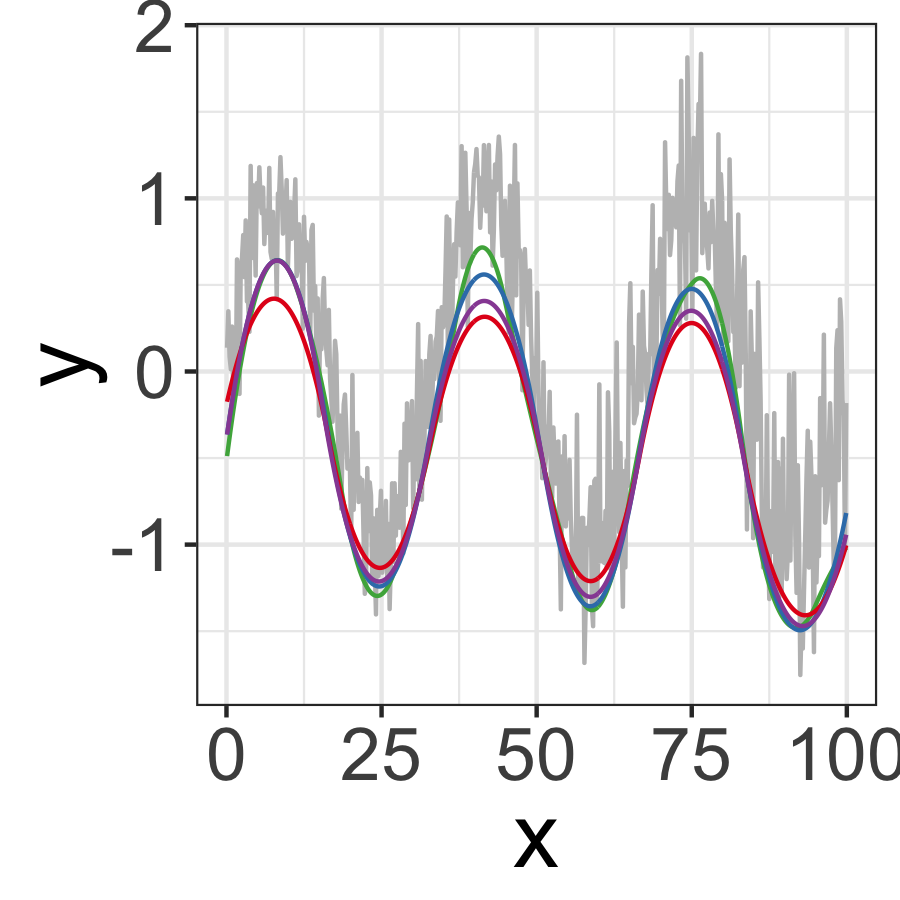
\includegraphics[width = 0.25\linewidth]{Figures/BIC_data.png}
	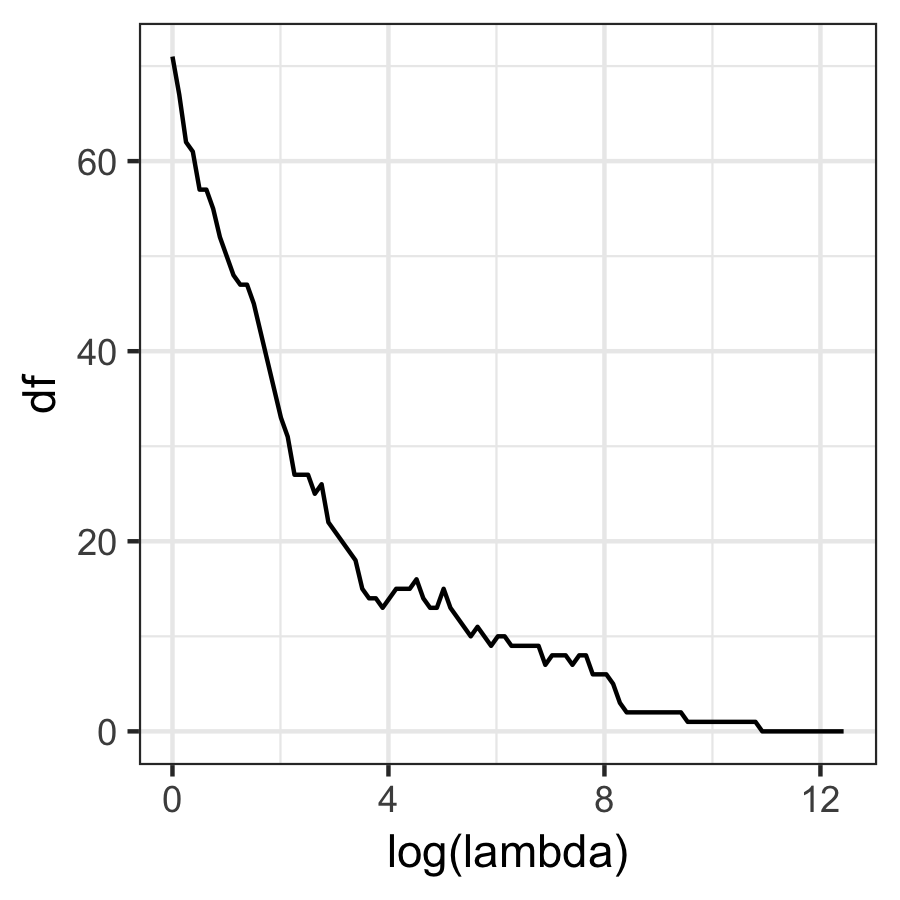
\includegraphics[width = 0.25\linewidth]{Figures/df_by_lambda.png}
	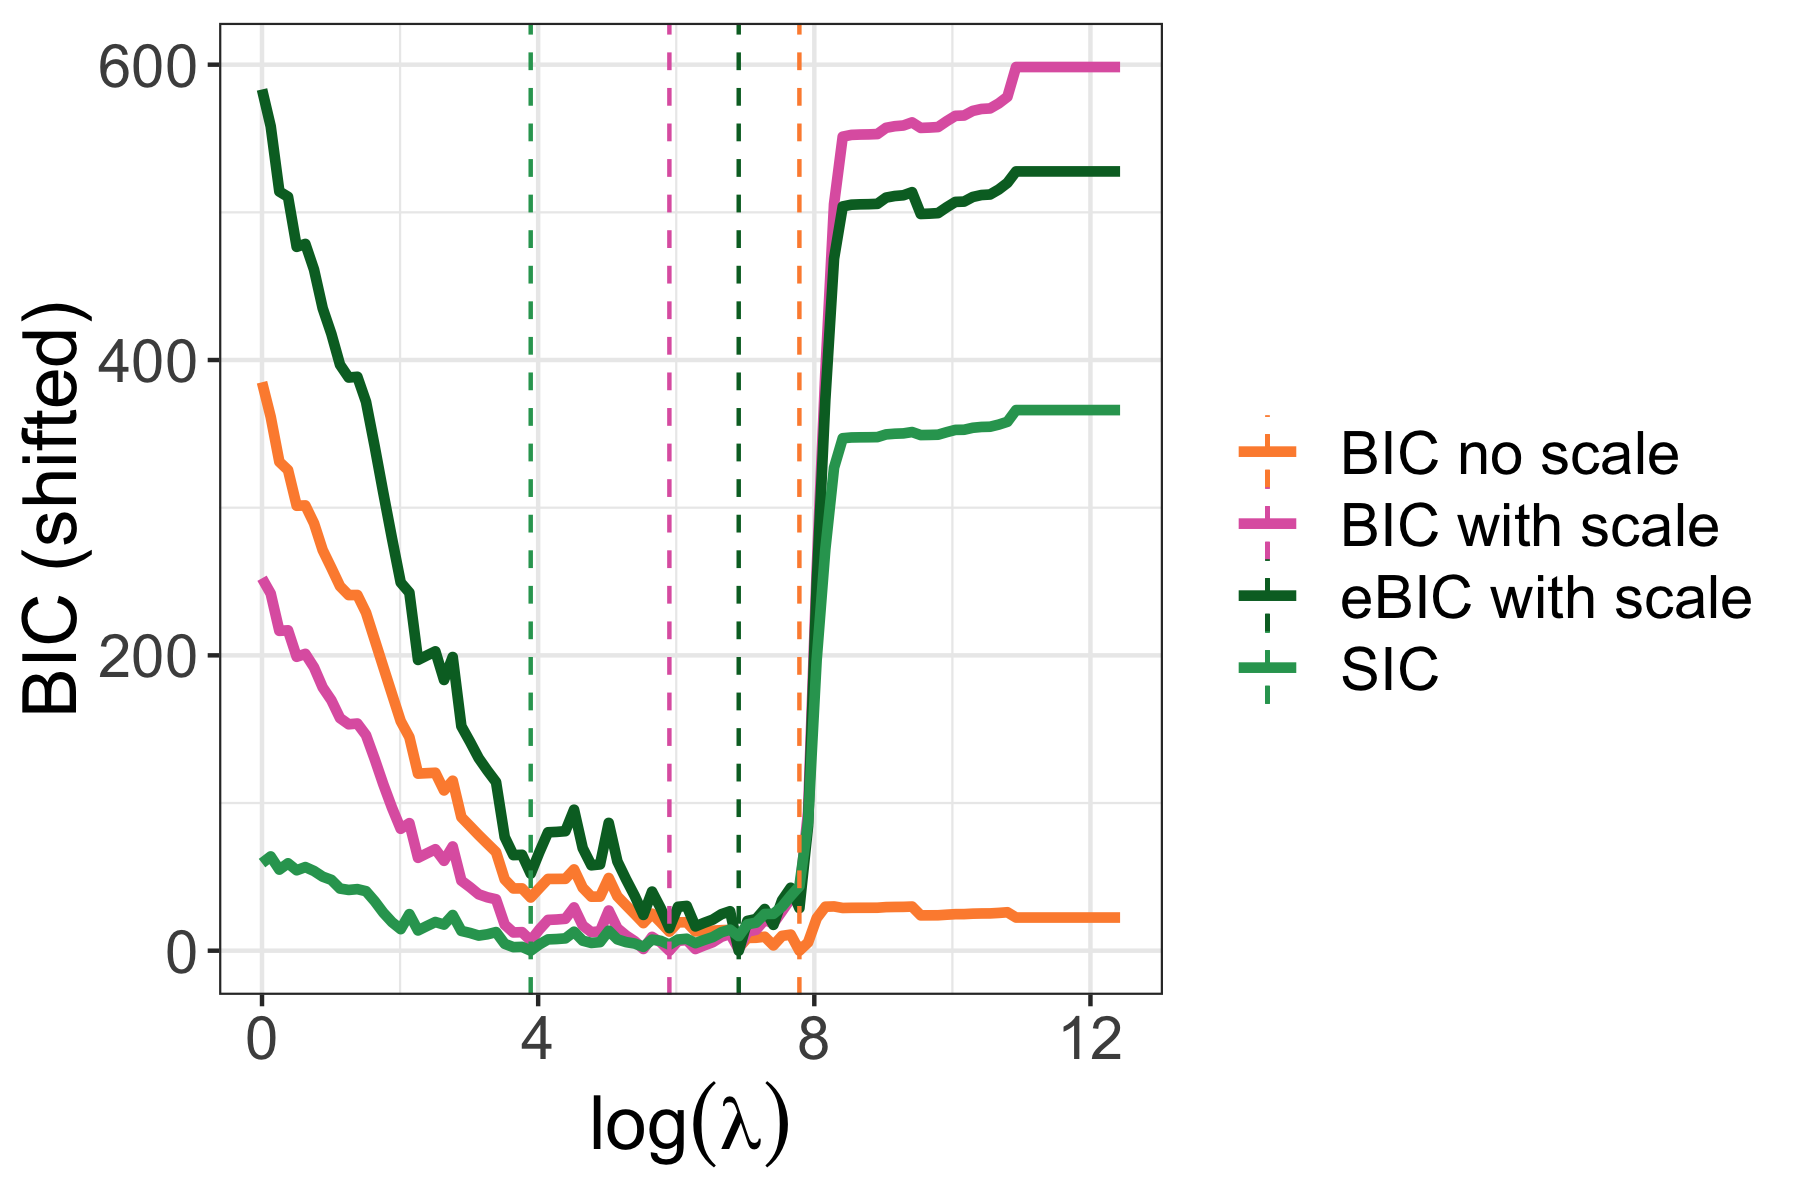
\includegraphics[width = 0.5\linewidth]{Figures/BIC_by_lambda.png}
\end{figure}

\subsection*{Design}
Three simulation designs from \cite{Racine2017} were considered. For all designs $X_i$ was generated as a uniformly spaced sequence in $[0,1]$ and the response $Y$ was generated as 
$$Y_i = sin(2\pi x_i) + \epsilon_i(x_i)$$
The three error distributions considered were 
\begin{itemize}
 \item Gaussian: $\epsilon_i(x_i) \sim N\left(0, \left(\frac{1+x_i^2}{4}\right)^2\right)$
 \item Beta: $\epsilon_i \sim Beta(1, 11-10x_i)$
\item Mixed normal: $\epsilon_i$ is simulated from a mixture of $N(-1,1)$ and  $N(1,1)$ with mixing probability $x_i$.
\end{itemize}
\begin{figure}
\caption{Simulated data with true quantiles $\tau \in \{0.01, 0.05, 0.25, 0.5, .75, 0.95, 0.99\}$}	
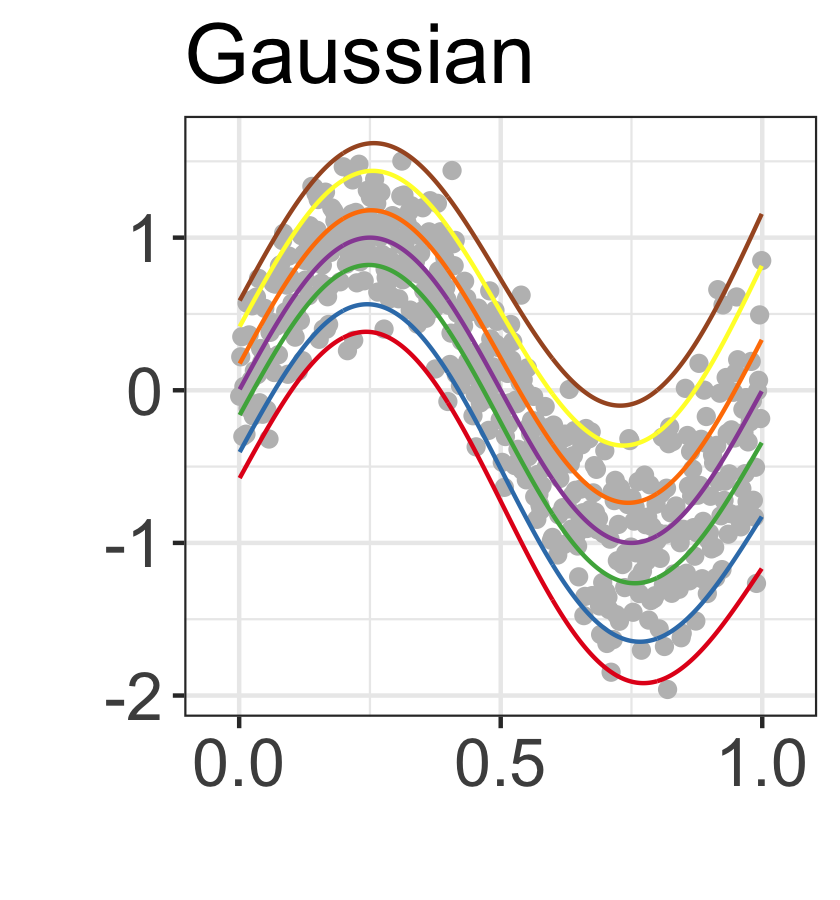
\includegraphics[width=.3\linewidth]{Figures/gaus.png}
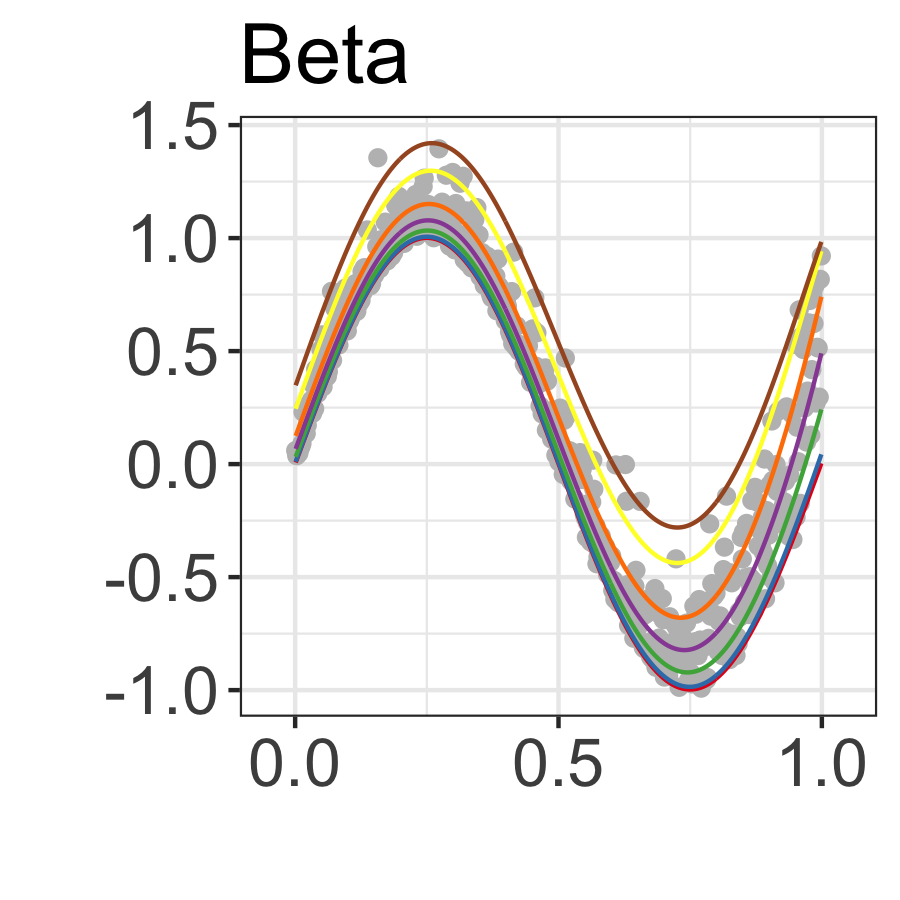
\includegraphics[width=.3\linewidth]{Figures/shapebeta.png}
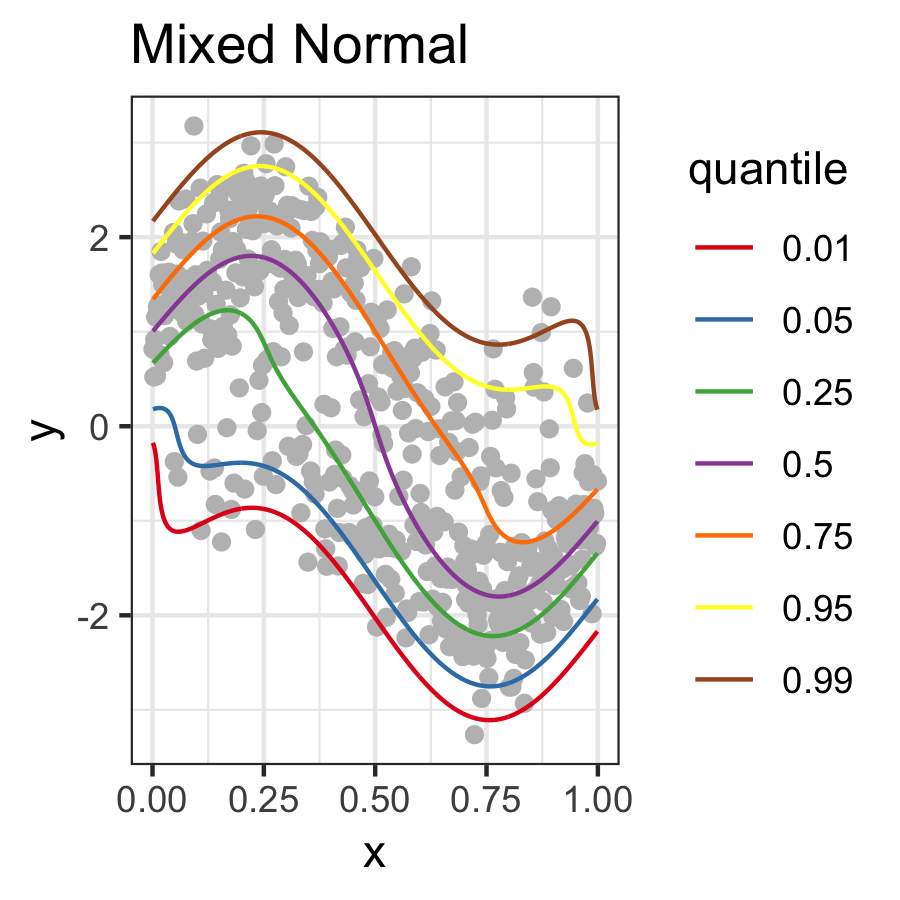
\includegraphics[width=.3\linewidth]{Figures/mixednorm.png}
\end{figure}

100 datasets were generated of sizes 300, 500 and 1000. The MSE was calculated as $\frac{1}{n}\sum_i (\hat{q}_{\tau}(x_i) - q_\tau(x_i))^2$. The plots below show the mean MSE $\pm$ twice the standard error by method, quantile level and sample size. 
	 
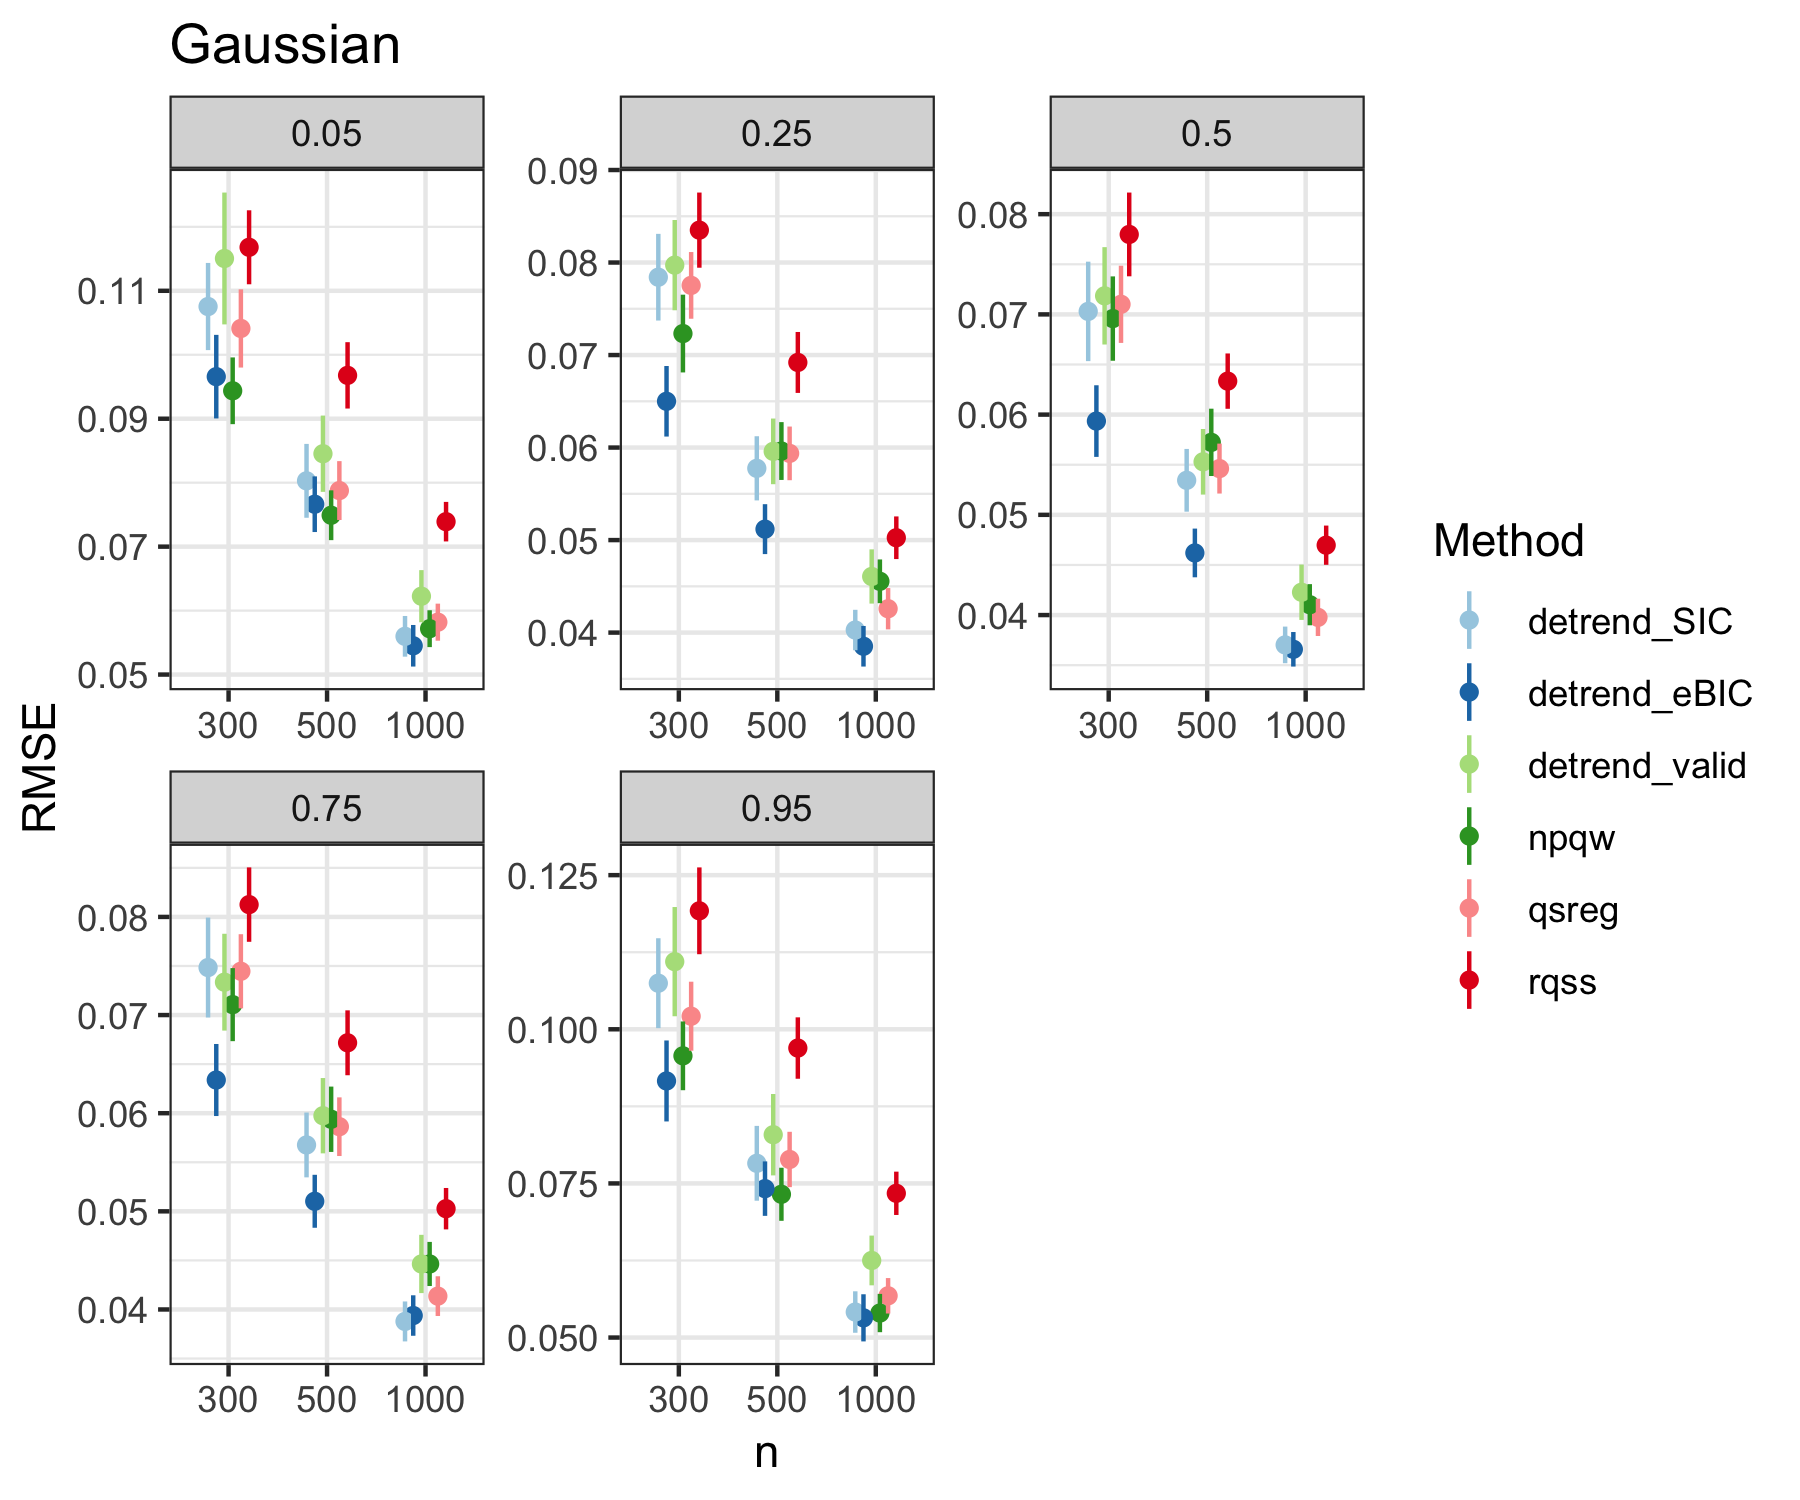
\includegraphics[width=\linewidth]{Figures/gaus_mse.png}	

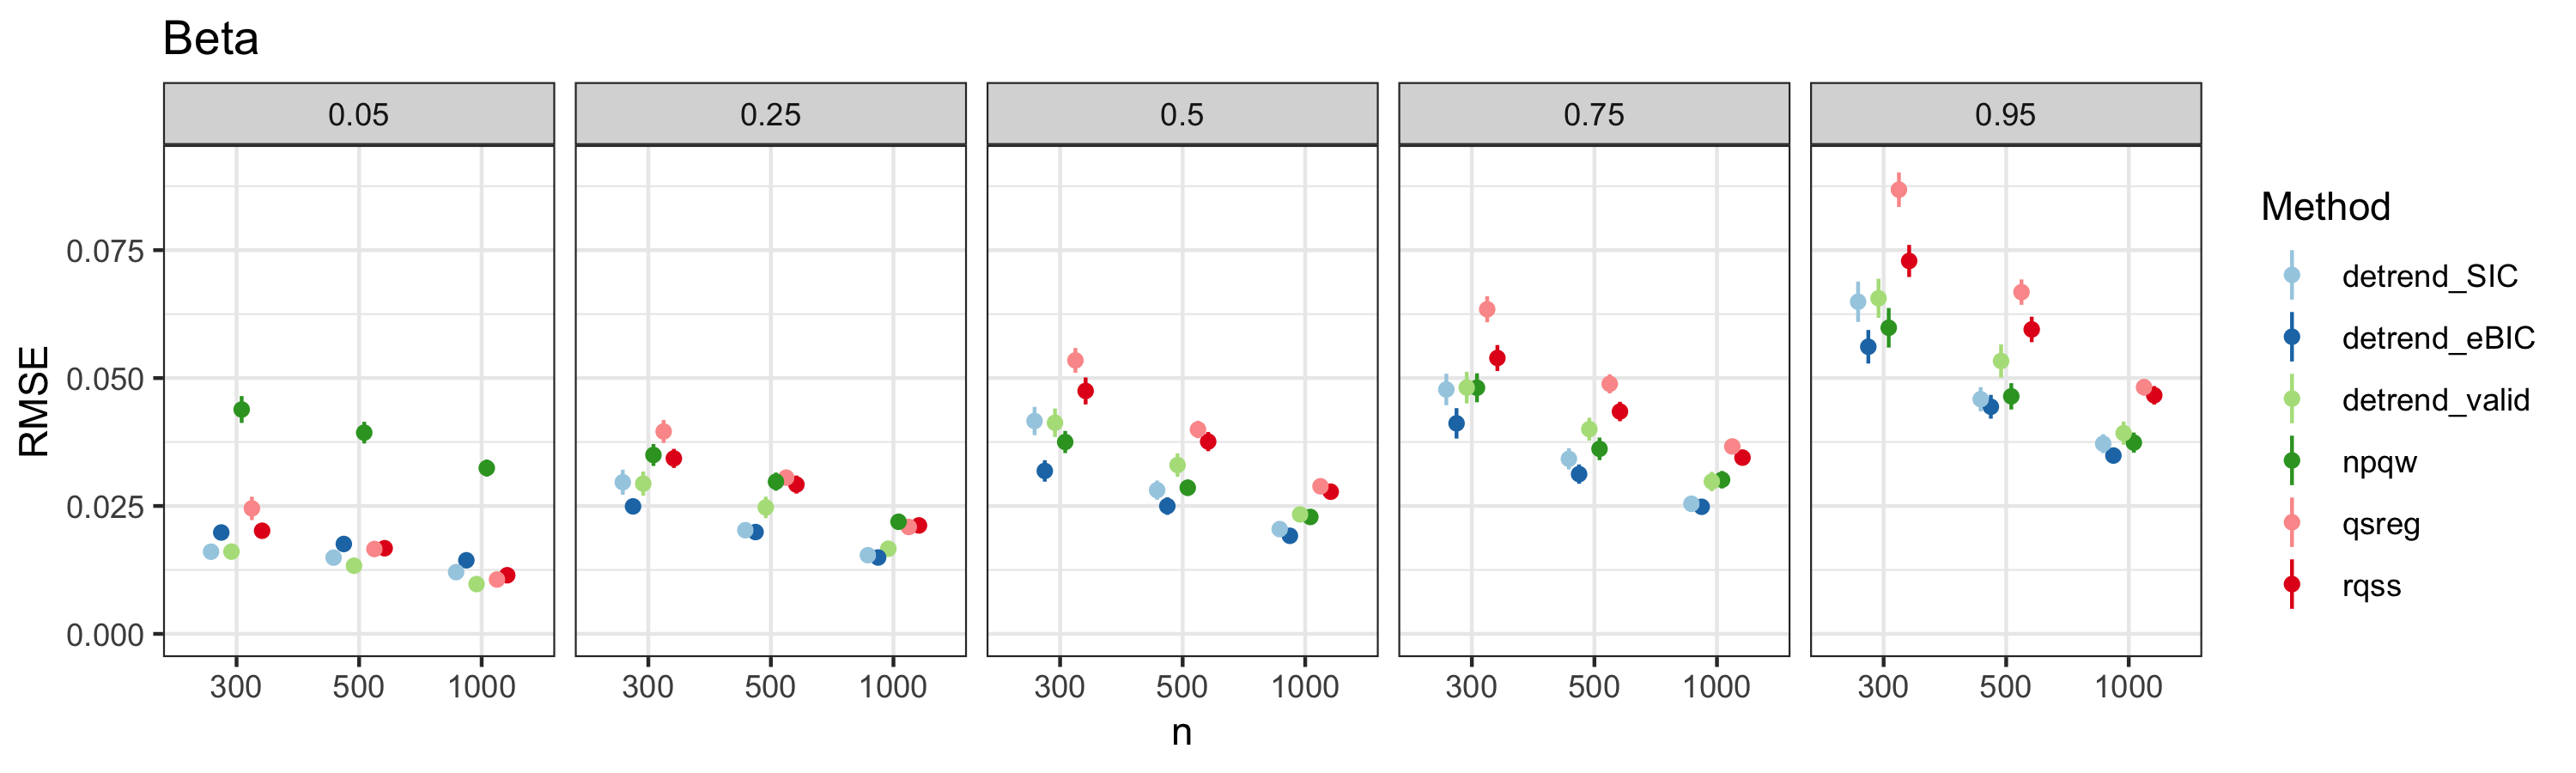
\includegraphics[width=\linewidth]{Figures/shapebeta_mse.png}

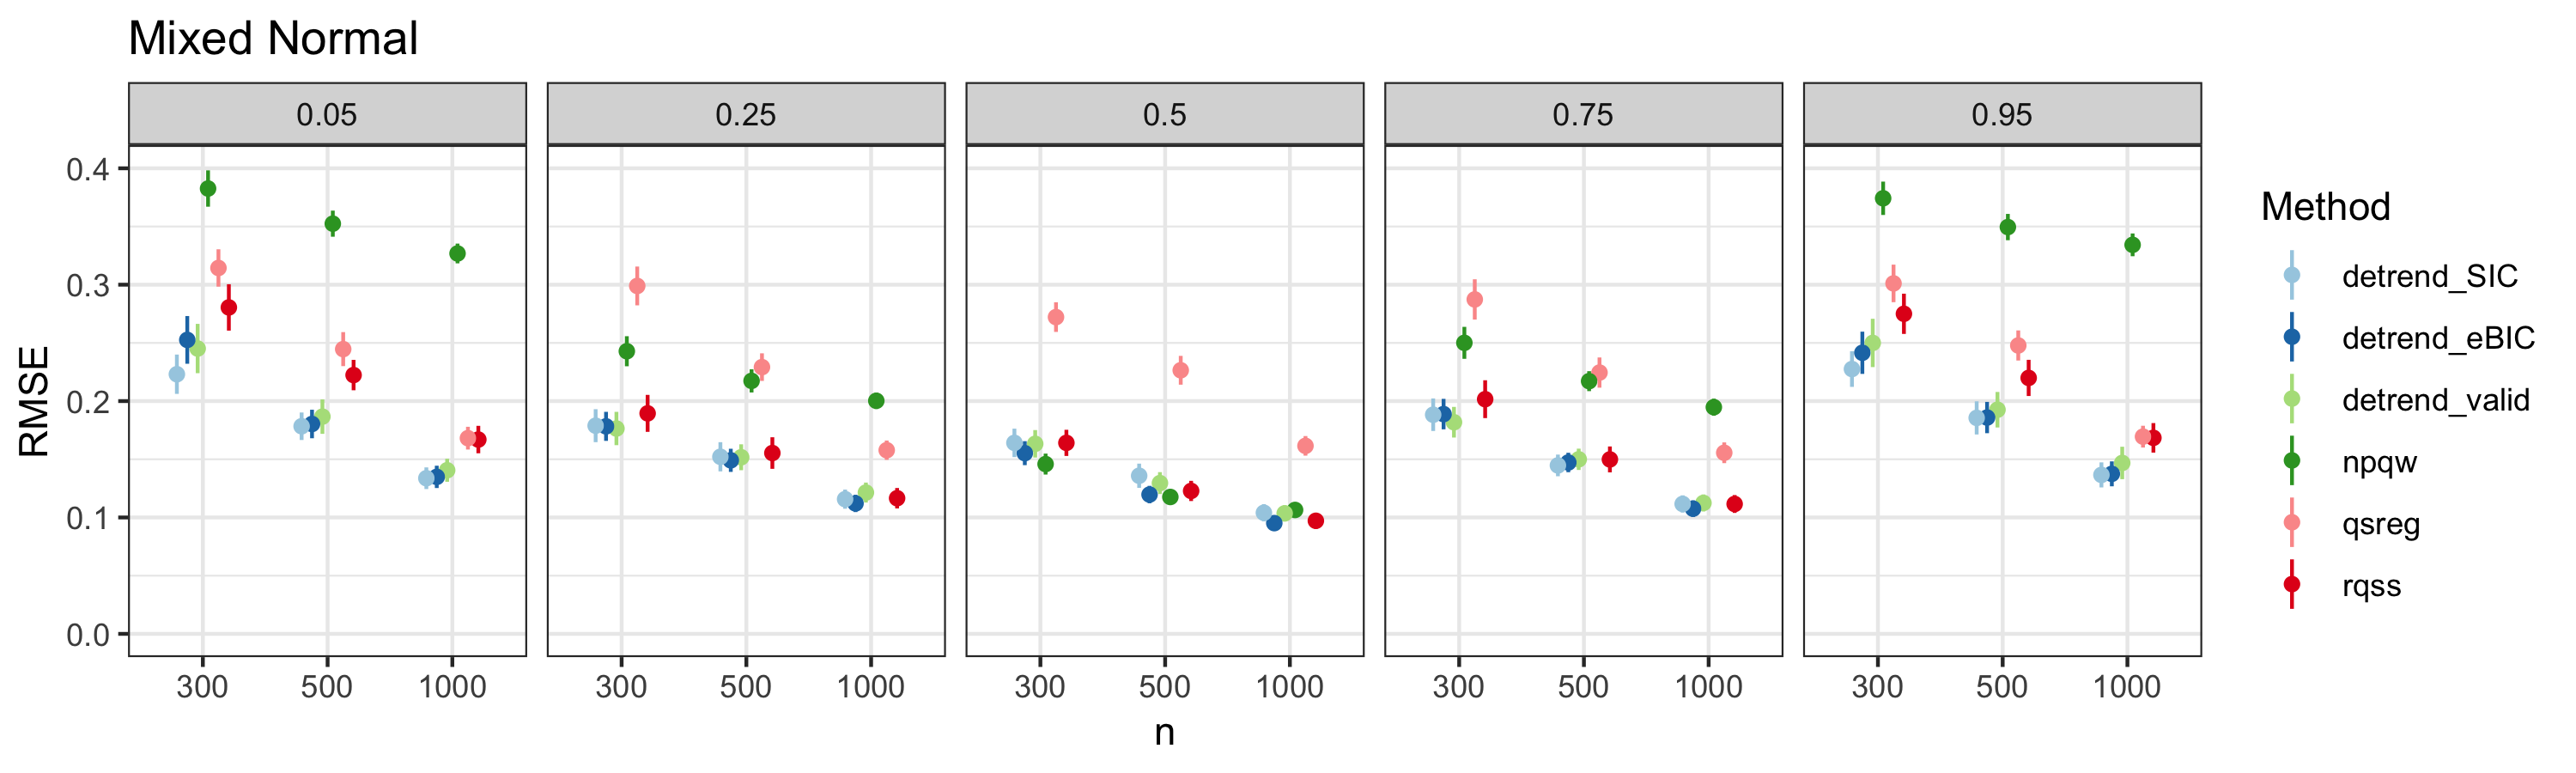
\includegraphics[width=\linewidth]{Figures/mixednorm_mse.png}


\section{Peaks Simulation}
We use another simulation design based on the applied problem we aim to solve. We assume that the measured data can be represented by 
\begin{equation}
Y(t) = s(t) + b(t) + \epsilon
\end{equation} 
where $s(t)$ is the true signal at time $t$, $b(t)$ is the drift component that varies smoothly over time and $\epsilon \sim N(0, \sigma^2)$ is an error component. We assume $t$ is a uniformly spaced sequence between 0 and 1. We generate $b(t)$ using a cubic natural spline basis function with degrees of freedom sampled from $n/50$ to $n/25$ with equal probability, and coefficients drawn from an exponential distribution with rate 1. The true signal function is assumed to be zero with Gaussian peaks. The number of peaks is sampled from $n/100$ to $n/50$ with equal probability with centers uniformly distributed between 0.1 and 0.9 and bandwidths uniformly distributed between $1/n$ and $5/n$ and areas uniformly distributed between 0 and $20/n$. One hundred datasets were generated for $n=\{300,500,1000, 5000\}$. We compare the methods ability to estimate the true quantiles of $b(t) + \epsilon$  for $\tau \in \{0.01, 0.05, 0.1\}$ and calculate the RMSE. 

\begin{figure}
	\caption{Example of simulated peaks, baseline, and observed measurements.}
	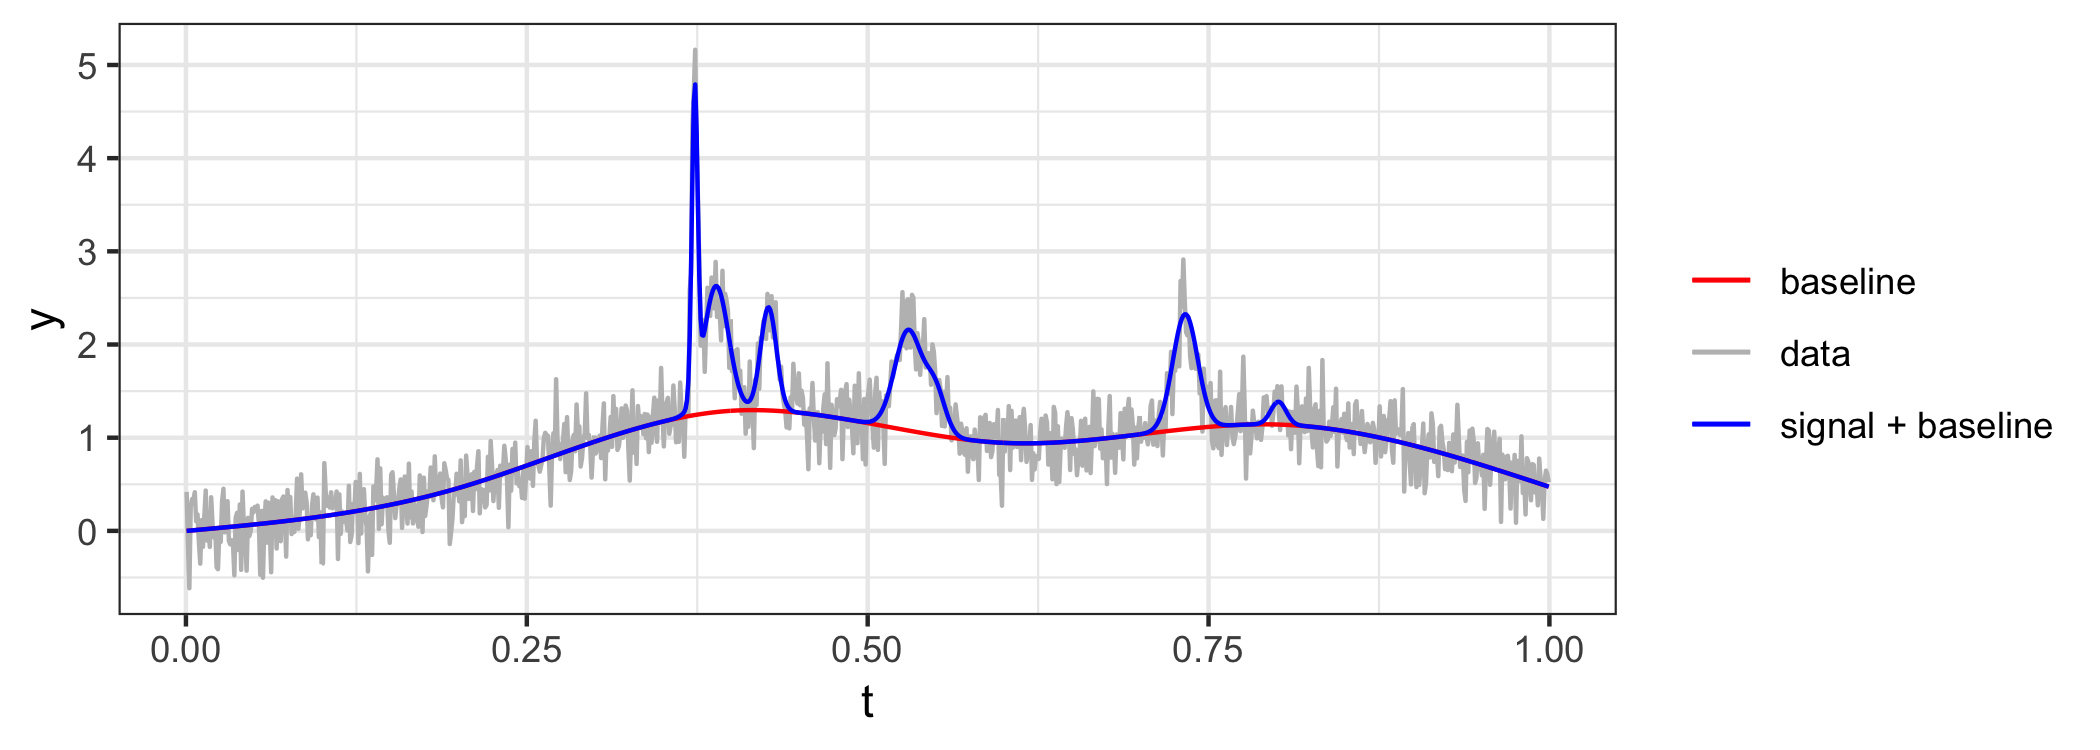
\includegraphics[width = \linewidth]{Figures/ex_peaks.png}
\end{figure}



\begin{figure}[h!]
	\caption{RMSEs compared to the simulated baseline function.}
	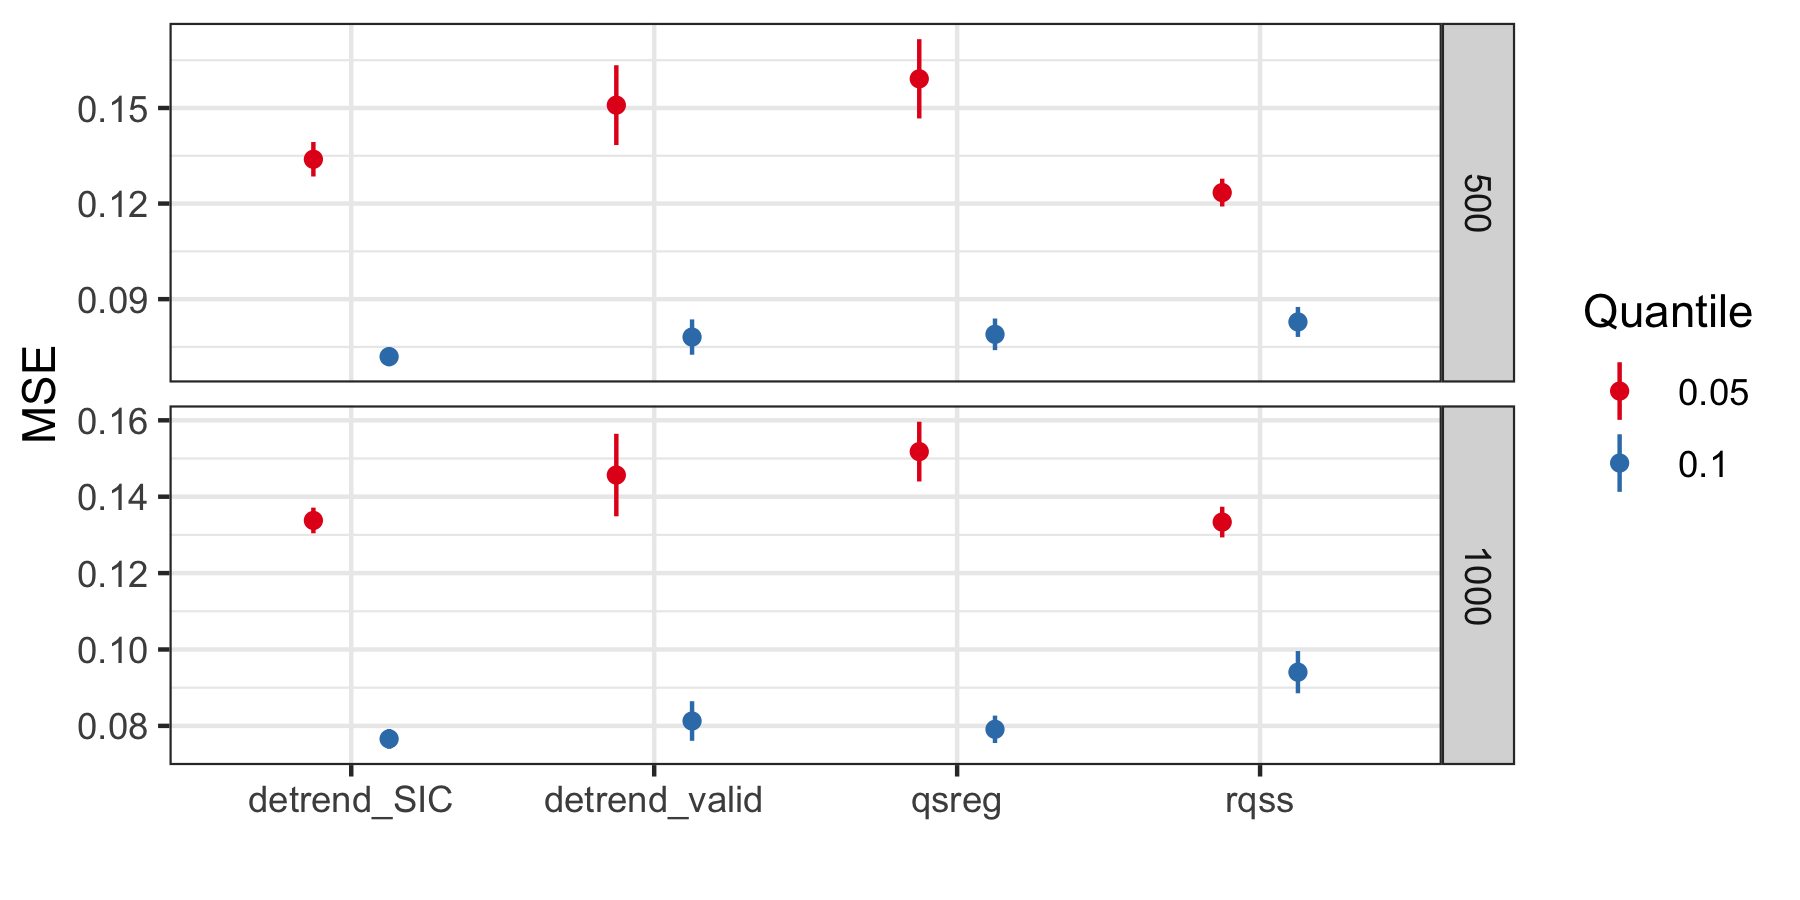
\includegraphics[width = \linewidth]{Figures/peaks_mse.png}
\end{figure}



\section{Application}

\begin{figure}
	\caption{Example of simulated peaks, baseline, and observed measurements.}
	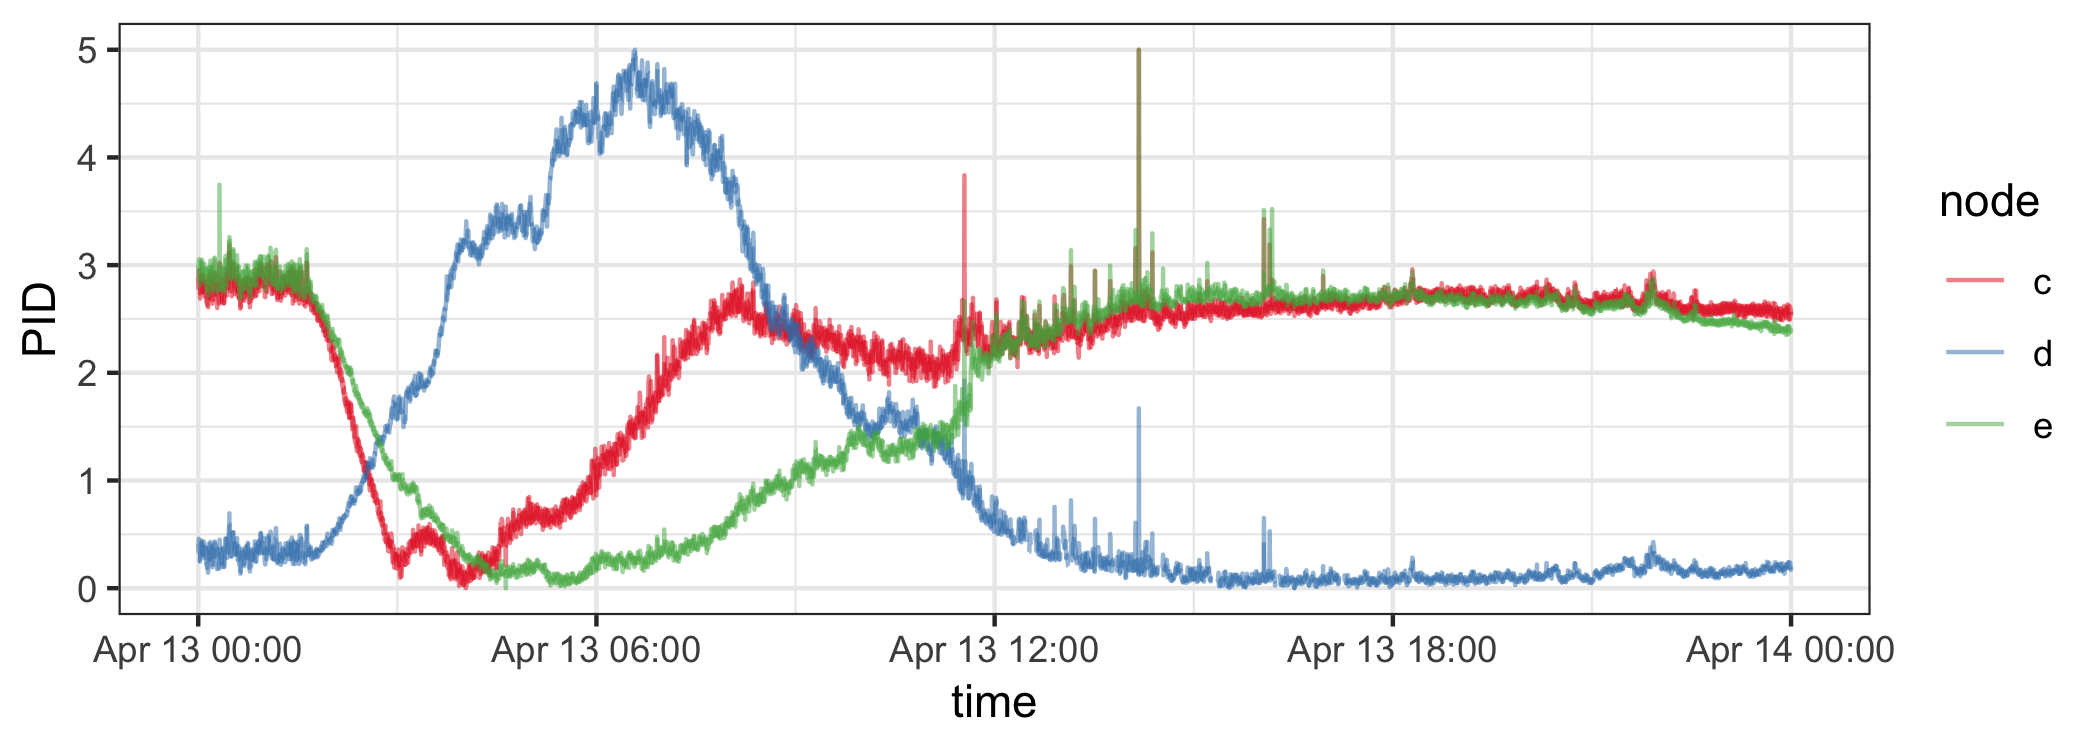
\includegraphics[width = \linewidth]{Figures/uncorrected_data.png}
	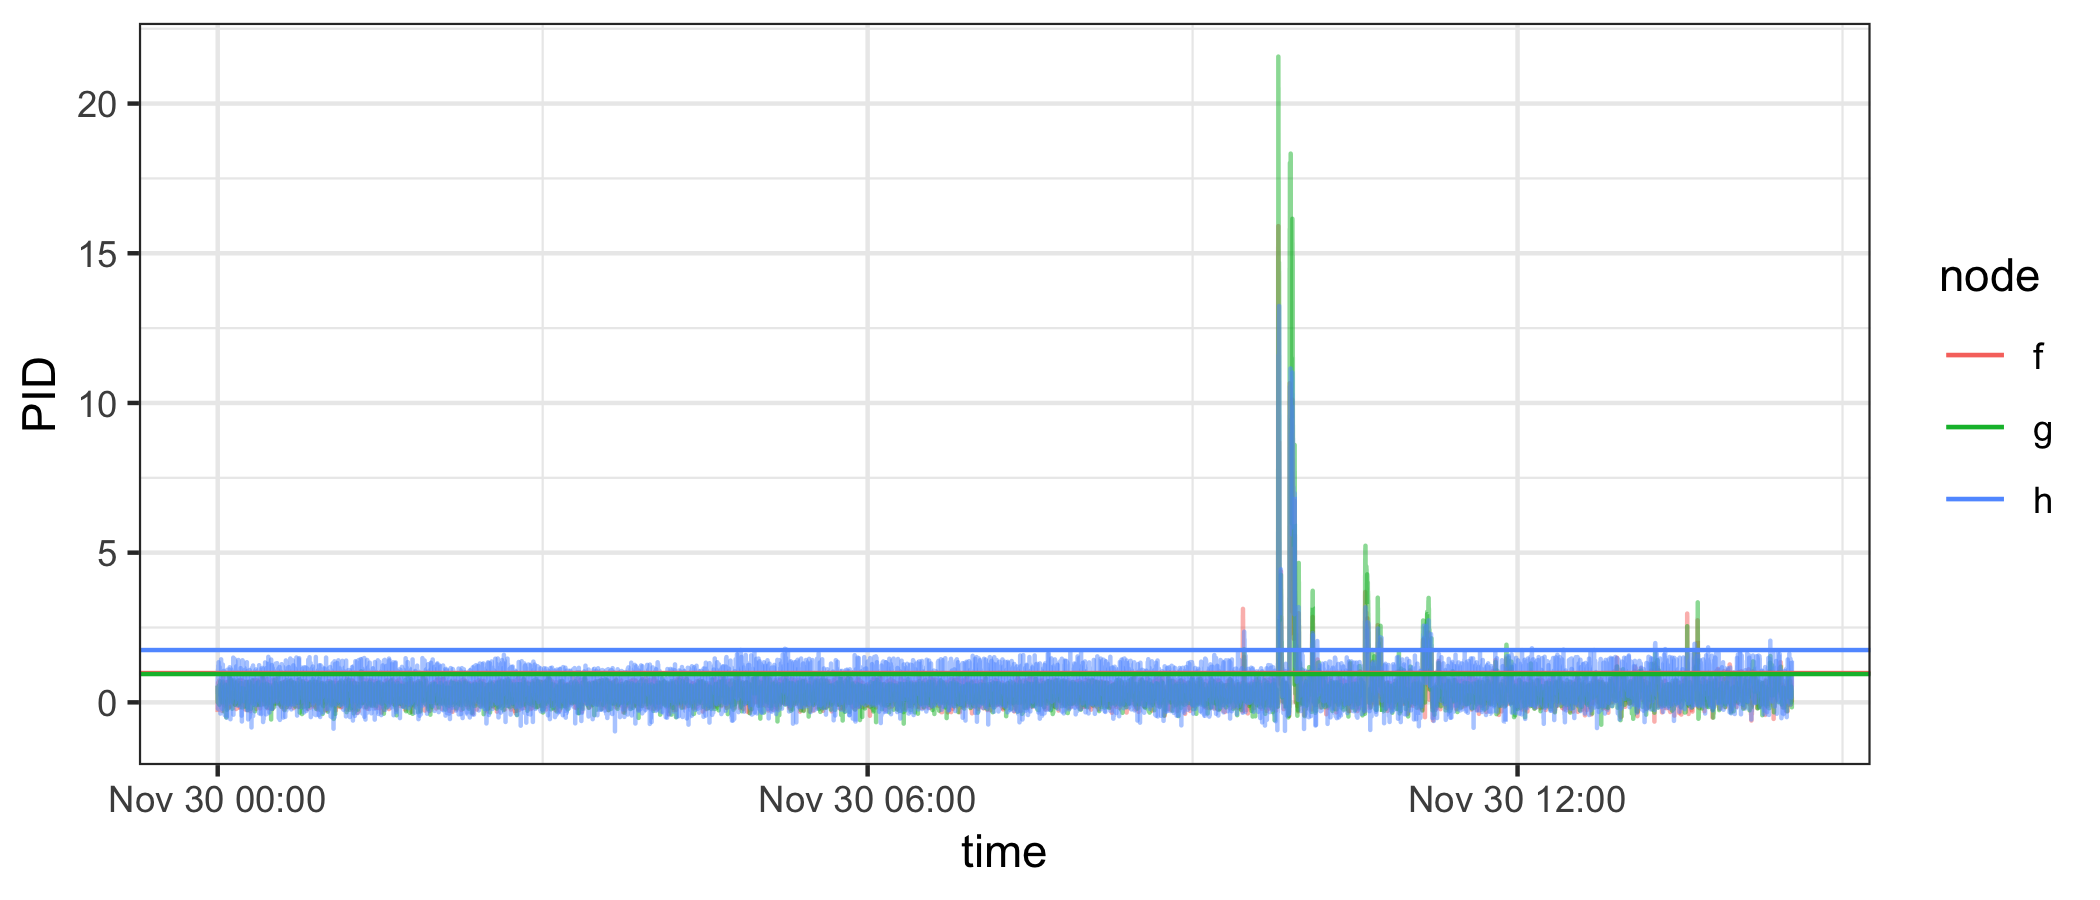
\includegraphics[width = \linewidth]{Figures/corrected_data.png}
	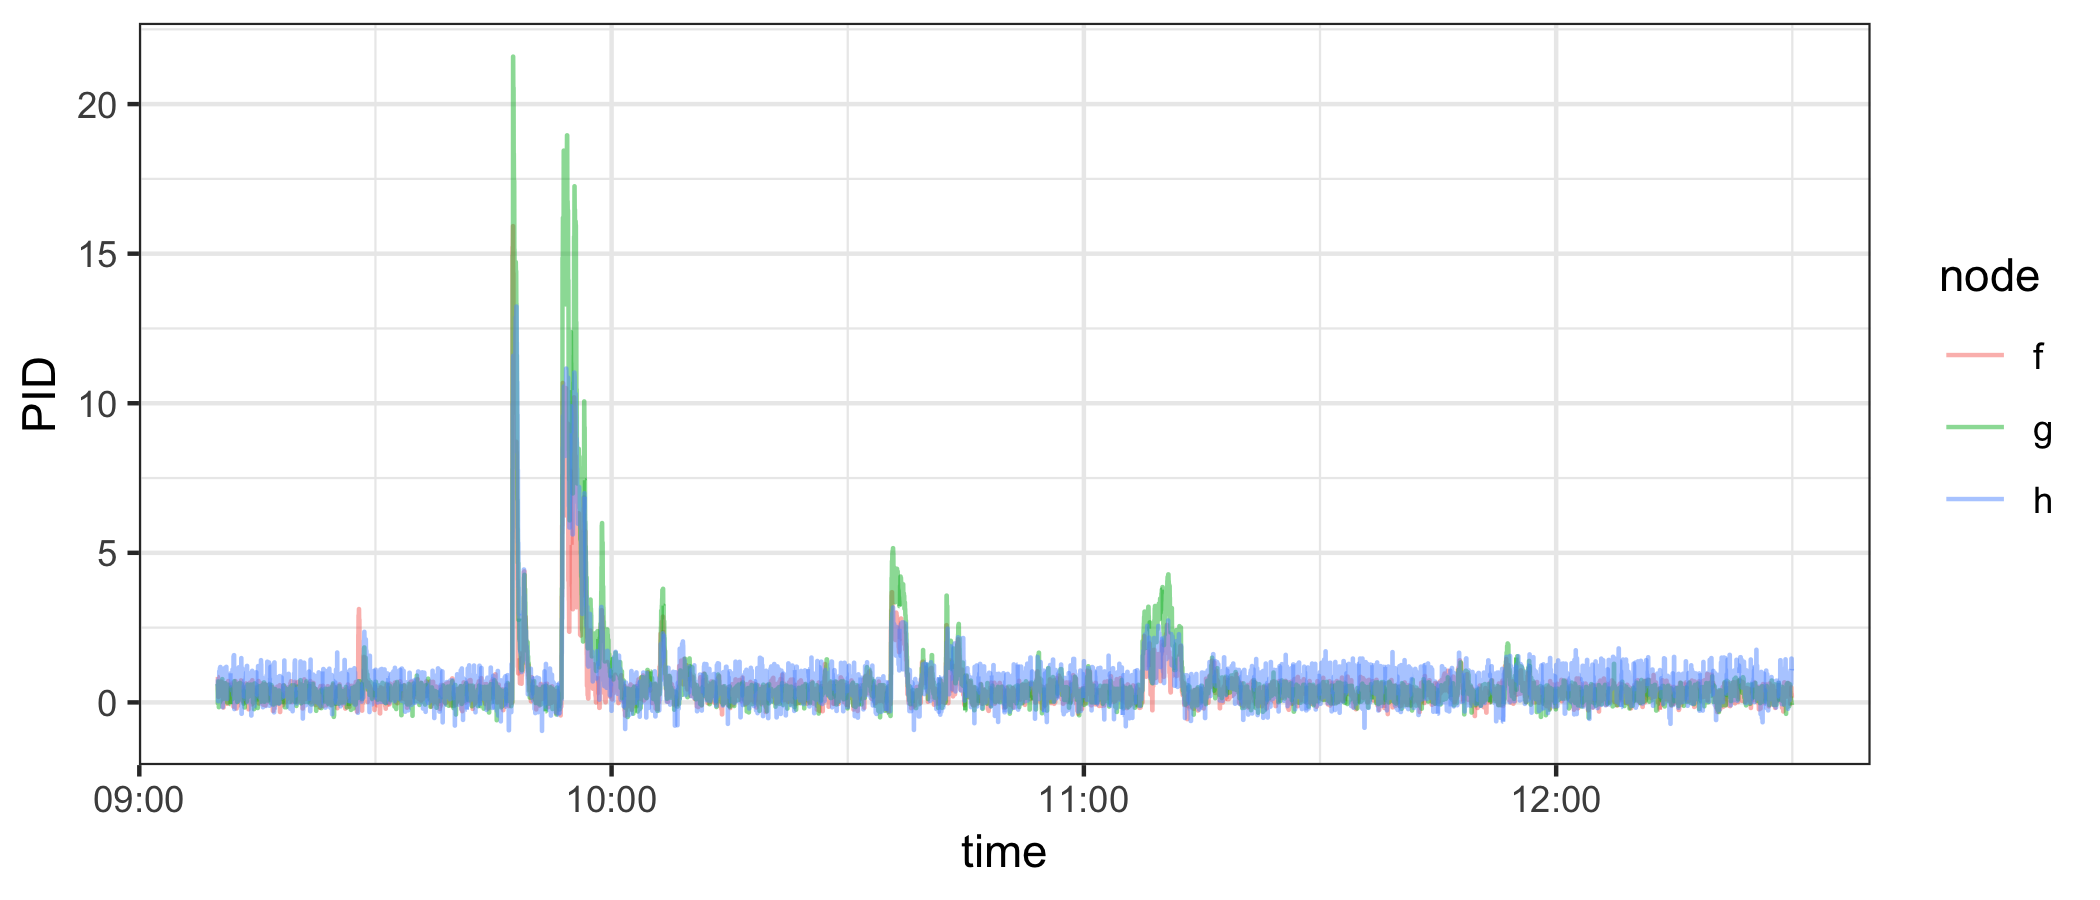
\includegraphics[width = \linewidth]{Figures/corrected_zoom_data.png}
\end{figure}

\pagebreak


\bibliographystyle{asa}
\bibliography{detrendify}
\end{document}